% defer/seqlock.tex

\section{Sequence Locks}
\label{sec:defer:Sequence Locks}

\begin{figure}[tb]
\begin{center}
\resizebox{3in}{!}{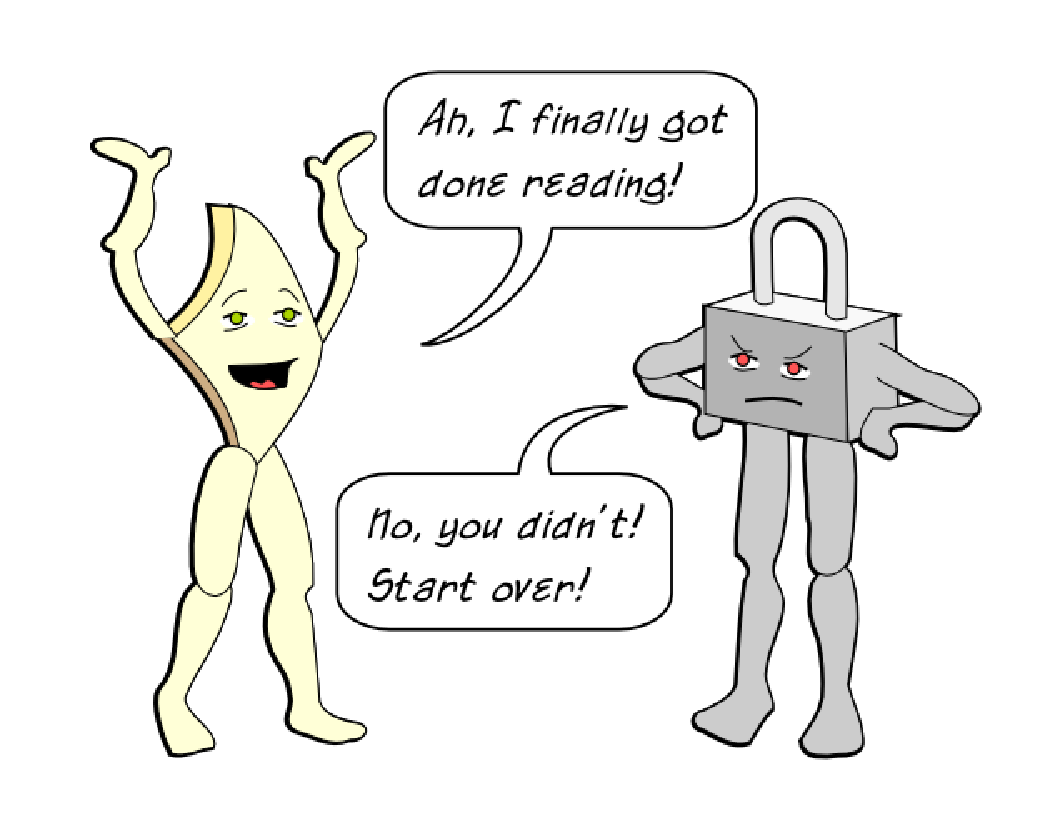
\includegraphics{cartoons/2013_Start-over}}
\end{center}
\caption{Reader And Uncooperative Sequence Lock}
\label{fig:defer:Reader And Uncooperative Sequence Lock}
\end{figure}

Sequence locks are used in the Linux kernel for read-mostly data that
must be seen in a consistent state by readers.
However, unlike reader-writer locking, readers do not exclude writers.
Instead, sequence locks force readers to
\emph{retry} an operation if they detect activity from a concurrent writer.
As can be seen from
Figure~\ref{fig:defer:fig:defer:Reader And Uncooperative Sequence Lock},
it is important to design code using sequence locks so that readers
very rarely need to retry.

\QuickQuiz{}
	Why isn't this sequence-lock discussion in Chapter~\ref{chp:Locking},
	you know, the one on \emph{locking}?
\QuickQuizAnswer{
	The sequence-lock mechanism is really a combination of two
	separate synchronization mechanisms, sequence counts and
	locking.
	In fact, the sequence-count mechanism is available separately
	in the Linux kernel via the
	\co{write_seqcount_begin()} and \co{write_seqcount_end()}
	primitives.

	However, the combined \co{write_seqlock()} and
	\co{write_sequnlock()} primitives are used much more heavily
	in the Linux kernel.
	More importantly, many more people will understand what you
	mean if you say ``sequence lock'' than if you say
	``sequence count''.

	So this section is entitled ``Sequence Locks'' so that people
	will understand what it is about just from the title, and
	it appears in the ``Deferred Processing'' because (1) of the
	emphasis on the ``sequence count'' aspect of ``sequence locks''
	and (2) because a ``sequence lock'' is much more than merely
	a lock.
} \QuickQuizEnd

\begin{figure}[bp]
{ \scriptsize
\begin{verbatim}
  1 do {
  2   seq = read_seqbegin(&test_seqlock);
  3   /* read-side access. */
  4 } while (read_seqretry(&test_seqlock, seq));
\end{verbatim}
}
\caption{Sequence-Locking Reader}
\label{fig:defer:Sequence-Locking Reader}
\end{figure}

\begin{figure}[bp]
{ \scriptsize
\begin{verbatim}
  1 write_seqlock(&test_seqlock);
  2 /* Update */
  3 write_sequnlock(&test_seqlock);
\end{verbatim}
}
\caption{Sequence-Locking Writer}
\label{fig:defer:Sequence-Locking Writer}
\end{figure}

The key component of sequence locking is the sequence number, which has
an even value in the absence of writers and an odd value if there
is an update in progress.
Readers can then snapshot the value before and after each access.
If either snapshot has an odd value, or if the two snapshots differ,
there has been a concurrent update, and the reader must discard
the results of the access and then retry it.
Readers use the \co{read_seqbegin()} and \co{read_seqretry()}
functions, as shown in Figure~\ref{fig:defer:Sequence-Locking Reader},
when accessing data protected by a sequence lock.
Writers must increment the value before and after each update,
and only one writer is permitted at a given time.
Writers use the \co{write_seqlock()} and \co{write_sequnlock()}
functions, as shown in Figure~\ref{fig:defer:Sequence-Locking Writer},
when updating data protected by a sequence lock.

Sequence-lock-protected data can have an arbitrarily large number of
concurrent readers, but only one writer at a time.
Sequence locking is used in the Linux kernel to protect calibration
quantities used for timekeeping.
It is also used in pathname traversal to detect concurrent rename operations.

\QuickQuiz{}
	Can you use sequence locks as the only synchronization
	mechanism protecting a linked list supporting concurrent
	addition, deletion, and search?
\QuickQuizAnswer{
	One trivial way of accomplishing this is to surround all
	accesses, including the read-only accesses, with
	\co{write_seqlock()} and \co{write_sequnlock()}.
	Of course, this solution also prohibits all read-side
	parallelism, and furthermore could just as easily be implemented
	using simple locking.

	If you do come up with a solution that uses \co{read_seqbegin()}
	and \co{read_seqretry()} to protect read-side accesses, make
	sure that you correctly handle the following sequence of events:

	\begin{enumerate}
	\item	CPU~0 is traversing the linked list, and picks up a pointer
		to list element~A.
	\item	CPU~1 removes element~A from the list and frees it.
	\item	CPU~2 allocates an unrelated data structure, and gets
		the memory formerly occupied by element~A.
		In this unrelated data structure, the memory previously
		used for element~A's \co{->next} pointer is now occupied
		by a floating-point number.
	\item	CPU~0 picks up what used to be element~A's \co{->next}
		pointer, gets random bits, and therefore gets a
		segmentation fault.
	\end{enumerate}

	One way to protect against this sort of problem requires use
	of ``type-safe memory'', which will be discussed in
	Section~\ref{sec:defer:RCU is a Way of Providing Type-Safe Memory}.
	But in that case, you would be using some other synchronization
	mechanism in addition to sequence locks!
} \QuickQuizEnd

\begin{figure}[bp]
{ \scriptsize
\begin{verbatim}
  1 typedef struct {
  2   unsigned long seq;
  3   spinlock_t lock;
  4 } seqlock_t;
  5 
  6 static void seqlock_init(seqlock_t *slp)
  7 {
  8   slp->seq = 0;
  9   spin_lock_init(&slp->lock);
 10 }
 11 
 12 static unsigned long read_seqbegin(seqlock_t *slp)
 13 {
 14   unsigned long s;
 15 
 16 repeat:
 17   s = ACCESS_ONCE(slp->seq);
 18   smp_mb();
 19   if (unlikely(s & 1))
 20     goto repeat;
 21   return s;
 22 }
 23 
 24 static int read_seqretry(seqlock_t *slp,
 25                          unsigned long oldseq)
 26 {
 27   unsigned long s;
 28 
 29   smp_mb();
 30   s = ACCESS_ONCE(slp->seq);
 31   return s != oldseq;
 32 }
 33 
 34 static void write_seqlock(seqlock_t *slp)
 35 {
 36   spin_lock(&slp->lock);
 37   ++slp->seq;
 38   smp_mb();
 39 }
 40 
 41 static void write_sequnlock(seqlock_t *slp)
 42 {
 43   smp_mb();
 44   ++slp->seq;
 45   spin_unlock(&slp->lock);
 46 }
\end{verbatim}
}
\caption{Sequence-Locking Implementation}
\label{fig:defer:Sequence-Locking Implementation}
\end{figure}

A simple implementation of sequence locks is shown in
Figure~\ref{fig:defer:Sequence-Locking Implementation}
(\co{seqlock.h}).
The \co{seqlock_t} data structure is shown on lines~1-4, and contains
the sequence number along with a lock to serialize writers.
Lines~6-10 show \co{seqlock_init()}, which, as the name indicates,
initializes a \co{seqlock_t}.

Lines~12-22 show \co{read_seqbegin()}, which begins a sequence-lock
read-side critical section.
Line~17 takes a snapshot of the sequence counter, and line~18 orders
this snapshot operation before the caller's critical section.
Line~19 checks to see if the snapshot is odd, indicating that there
is a concurrent writer, and, if so, line~20 jumps back to the beginning.
Otherwise, line~21 returns the value of the snapshot, which the caller
will pass to a later call to \co{read_seqretry()}.

\QuickQuiz{}
	Why bother with the check on line~19 of
	\co{read_seqbegin()} in
	Figure~\ref{fig:defer:Sequence-Locking Implementation}?
	Given that a new writer could begin at any time, why not
	simply incorporate the check into line~31 of
	\co{read_seqretry()}?
\QuickQuizAnswer{
	That would be a legitimate implementation.
	However, it would not save anything to move the check down
	to \co{read_seqretry()}: There would be roughly the same number
	of instructions.
	Furthermore, the reader's accesses from its doomed read-side
	critical section could inflict overhead on the writer in
	the form of cache misses.
	We can avoid these cache misses by placing the check in
	\co{read_seqbegin()} as shown on line~19 of
	Figure~\ref{fig:defer:Sequence-Locking Implementation}.
} \QuickQuizEnd

Lines~24-32 show \co{read_seqretry()}, which returns true if there
were no writers present since the time of the corresponding
call to \co{read_seqbegin()}.
Line~29 orders the caller's prior critical section before line~30's
fetch of the new snapshot of the sequence counter.
Finally, line~30 checks that the sequence counter has not changed,
in other words, that there has been no writer, and returns true if so.

\QuickQuiz{}
	Why is the \co{smp_mb()} on line~29 of
	Figure~\ref{fig:defer:Sequence-Locking Implementation}
	needed?
\QuickQuizAnswer{
	If it was omitted, both the compiler and the CPU would be
	within their rights to move the critical section preceding
	the call to \co{read_seqretry()} down below this function.
	This would prevent the sequence lock from protecting the
	critical section.
	The \co{smp_mb()} primitive prevents such reordering.
} \QuickQuizEnd

\QuickQuiz{}
	What prevents sequence-locking updaters from starving readers?
\QuickQuizAnswer{
	Nothing.
	This is one of the weaknesses of sequence locking, and as a
	result, you should use sequence locking only in read-mostly
	situations.
	Unless of course read-side starvation is acceptable in your
	situation, in which case, go wild with the sequence-locking updates!
} \QuickQuizEnd

Lines~34-39 show \co{write_seqlock()}, which simply acquires the lock,
increments the sequence number, and executes a memory barrier to ensure
that this increment is ordered before the caller's critical section.
Lines~41-46 show \co{write_sequnlock()}, which executes a memory barrier
to ensure that the caller's critical section is ordered before the
increment of the sequence number on line~44, then releases the lock.

\QuickQuiz{}
	What if something else serializes writers, so that the lock
	is not needed?
\QuickQuizAnswer{
	In this case, the \co{->lock} field could be omitted, as it
	is in \co{seqcount_t} in the Linux kernel.
} \QuickQuizEnd

\QuickQuiz{}
	Why isn't \co{seq} on line 2 of
	Figure~\ref{fig:defer:Sequence-Locking Implementation}
	\co{unsigned} rather than \co{unsigned long}?
	After all, if \co{unsigned} is good enough for the Linux
	kernel, shouldn't it be good enough for everyone?
\QuickQuizAnswer{
	Not at all.
	The Linux kernel has a number of special attributes that allow
	it to ignore the following sequence of events:
	\begin{enumerate}
	\item	Thread 0 executes \co{read_seqbegin()}, picking up
		\co{->seq} in line~17, noting that the value is even,
		and thus returning to the caller.
	\item	Thread 0 starts executing its read-side critical section,
		but is then preempted for a long time.
	\item	Other threads repeatedly invoke \co{write_seqlock()} and
		\co{write_sequnlock()}, until the value of \co{->seq}
		overflows back to the value that Thread~0 fetched.
	\item	Thread 0 resumes execution, completing its read-side
		critical section with inconsistent data.
	\item	Thread 0 invokes \co{read_seqretry()}, which incorrectly
		concludes that Thread~0 has seen a consistent view of
		the data protected by the sequence lock.
	\end{enumerate}

	The Linux kernel uses sequence locking for things that are
	updated rarely, with time-of-day information being a case
	in point.
	This information is updated at most once per millisecond,
	so that seven weeks would be required to overflow the counter.
	If a kernel thread was preempted for seven weeks, the Linux
	kernel's soft-lockup code would be emitting warnings every two
	minutes for that entire time.

	In contrast, with a 64-bit counter, more than five centuries
	would be required to overflow, even given an update every
	\emph{nano}second.
	Therefore, this implementation uses a type for \co{->seq}
	that is 64 bits on 64-bit systems.
} \QuickQuizEnd

Both the read-side and write-side critical sections of a sequence lock
can be thought of as transactions, and sequence locking therefore
can be thought of as a limited form of transactional memory, which
will be discussed in Section~\ref{sec:future:Transactional Memory}.
The limitations of sequence locking are: (1)~Sequence locking restricts
updates and (2)~sequence locking does not permit traversal of pointers
to objects that might be freed by updaters.
These limitations are of course overcome by transactional memory, but
can also be overcome by combining other synchronization primitives
with sequence locking.

Sequence locks allow writers to defer readers, but not vice versa.
This can result in unfairness and even starvation
in writer-heavy workloads.
On the other hand, in the absence of writers, sequence-lock readers are
reasonably fast and scale linearly.
It is only human to want the best of both worlds: fast readers without
the possibility of starvation.
In addition, it would also be nice to overcome sequence locking's limitations
with pointers.
The following section presents a synchronization mechanism with exactly
these proporties.
